\section{Udvælgelse af gestik-par til at skifte musiknummer}
\label{TestresultaterSkiftMusiknummer}
%
Udvælgelsen af hvilket gestik-par, der skal knyttes til at skifte musiknummer frem og tilbage foretages på baggrund af testpersonernes udsagn. I \fullref{app:TestresultaterSkiftDaarlig} analyseres testpersonernes respons i forhold til hvilke gestik-par de mindst kan lide og på baggrund af den analyse ekskluderes gestik-par 2, gestik-par 4 og gestik-par 7 fra yderligere undersøgelser. Dette medfører at udvælgelsen af hvilket gestik-par, der skal knyttes til at skifte musiknummer kun foretages på gestik-par 1, gestik-par 3, gestik-par 5 og gestik-par 6.\blankline
%  
I nedenstående \autoref{tab:GestikParITopTreSkift} fremgår samtlige testpersoners top tre rangering, hvor der ikke er taget forbehold for hvorvidt testpersonerne har inkluderet et gestik-par, som der på baggrund af \fullref{app:TestresultaterSkiftDaarlig} er blevet ekskluderet.
%
\begin{table}[H]
	\centering
	\begin{tabular}{ | p{3cm} | p{3cm} | p{3cm} | p{3cm} |}
		\hline
		& 1. Plads & 2. Plads & 3. Plads \\ \hline
		Testperson 1 & Gestik-par 1 & Gestik-par 5 & Gestik-par 6 \\ \hline
		Testperson 2 & Gestik-par 1 & Gestik-par 5 & Gestik-par 3 \\ \hline
		Testperson 3 & Gestik-par 1 & Gestik-par 5 & Gestik-par 4 \\ \hline
		Testperson 4 & Gestik-par 2 & Gestik-par 5 & Gestik-par 3 \\ \hline
		Testperson 5 & Gestik-par 1 & Gestik-par 5 & Gestik-par 3 \\ \hline
		Testperson 6 & Gestik-par 1 & Gestik-par 3 & Gestik-par 6 \\ \hline 
		Testperson 7 & Gestik-par 1 & Gestik-par 7 & Gestik-par 3 \\ \hline
		Testperson 8 & Gestik-par 3 & Gestik-par 2 & Gestik-par 7 \\ \hline
		Testperson 9 & Gestik-par 5 & Gestik-par 1 & Gestik-par 3 \\ \hline
		Testperson 10 & Gestik-par 1 & Gestik-par 5 & Gestik-par 3 \\ \hline
		Testperson 11 & Gestik-par 5 & Gestik-par 6 & Gestik-par 4 \\ \hline
		Testperson 12 & Gestik-par 1 & Gestik-par 2 & Gestik-par 5 \\ \hline
		Testperson 13 & Gestik-par 6 & Gestik-par 5 & Gestik-par 4 \\ \hline
		Testperson 14 & Gestik-par 5 & Gestik-par 6 & Gestik-par 4 \\ \hline
		Testperson 15 & Gestik-par 1 & Gestik-par 2 & Gestik-par 5 \\ \hline
		Testperson 16 & Gestik-par 1 & Gestik-par 3 & Gestik-par 7 \\ \hline
		Testperson 17 & Gestik-par 2 & Gestik-par 3 & Gestik-par 4 \\ \hline
		Testperson 18 & Gestik-par 2 & Gestik-par 1 & Gestik-par 3 \\ \hline
	\end{tabular}
	\caption{Oversigt over samtlige testpersoners top tre i forbindelse med at skifte musiknummer.}
	\label{tab:GestikParITopTreSkift}
\end{table}
\noindent
%
Da der er tre gestik-par, som er blevet ekskluderet, kan ovenstående  \autoref{tab:GestikParITopTreSkift} med fordel opsummeres både i forhold til at fjerne de tre gestik-par men også i forhold til at opsummere hvor mange gange de fire tilbageværende gestik-par indgår i top tre rangeringen. 
%
\begin{table}[H]
	\centering
	\begin{tabular}{ | p{2.4cm} | p{2.4cm} | p{2.4cm} | p{2.4cm} |p{2.4cm}|}
		\hline
		& 1. Plads & 2. Plads & 3. Plads & I alt \\ \hline
		Gestik-par 1 & 10 & 2 & 0 & 12\\ \hline
		Gestik-par 3 & 1 & 3 & 7 & 11\\ \hline
		Gestik-par 5 & 3 & 7 & 2 & 12\\ \hline 
		Gestik-par 6 & 1 & 2 & 2 & 5\\ \hline
	\end{tabular}
	\caption{Oversigt over dels hvor mange gange hvert gestik-par indgår i samtlige testpersoners top tre i forbindelse med at skifte musiknummer og dels over hvor mange gange et gestik-par sammenlagt indgår i en top tre.}
	\label{tab:GestikParITopTreSkiftOversigt}
\end{table}
\noindent
%
Der er forskellige årsager til hvorfor de 10 testpersoner har rangeret gestik-par 1 på en første plads. Gestik-par 1 er illustreret på \autoref{fig:GestikPar1Skift}. Fire ud af de 10 testpersoner, forbinder gestik-par 1 med hvordan de normalvist interagerer med en tablet eller en smartphone, hvor de i forvejen er bekendt med swipe-bevægelsen, illustreret på \autoref{fig:GestikPar1Skift}. Blandt de fire er testperson 1, som ydermere kommenterer at i gestik-par 1 så er der intet besværligt håndtegn, hvilket går igen ved testperson 2 og testperson 10. Derudover foretrækker testperson 1 at der er en bevægelse for at skifte musiknummer, hvilket ligeledes bliver fortrukket af testperson 3 og testperson 5. Endvidere giver testperson 1 udtryk for at gestik-par 1 er naturlig, hvilket testperson 5 og testperson 6 ligeledes giver udtryk for. En anden gennemgående tendens er at fire testpersoner giver udtryk for at gestik-par 1 giver meningen. De fire testpersoner, som giver udtryk for at gestik-par 1 giver meningen er ikke de samme fire testpersoner, som forbinder gestik-par 1 med at swipe på en tablet eller en smartphone. Derudover beskriver de 10 testpersoner gestik-par 1 som værende; simpel, intuitiv, logisk, enkel, nem at udføre og nem at forstå. Testperson 6 påpeger et potentielt problem når der skal skiftes tilbage til det forrige musiknummer og der ikke skiftes tilbage for at genspille musiknummeret. Det er selvfølgelig noget, der skal tages højde for, men som det er kendt fra blandt andet iTunes; så hvis der skiftes tilbage inden for relativt kort tid, så er det det forrige musiknummer, som afspilles og ikke det pågældende musiknummer som genstartes. Det kan være en løsning at gøre implementere samme princip i Bang $\&$ Olufsen's fremtidige musikanlæg. 
%
\begin{figure}[H]
	\centering
	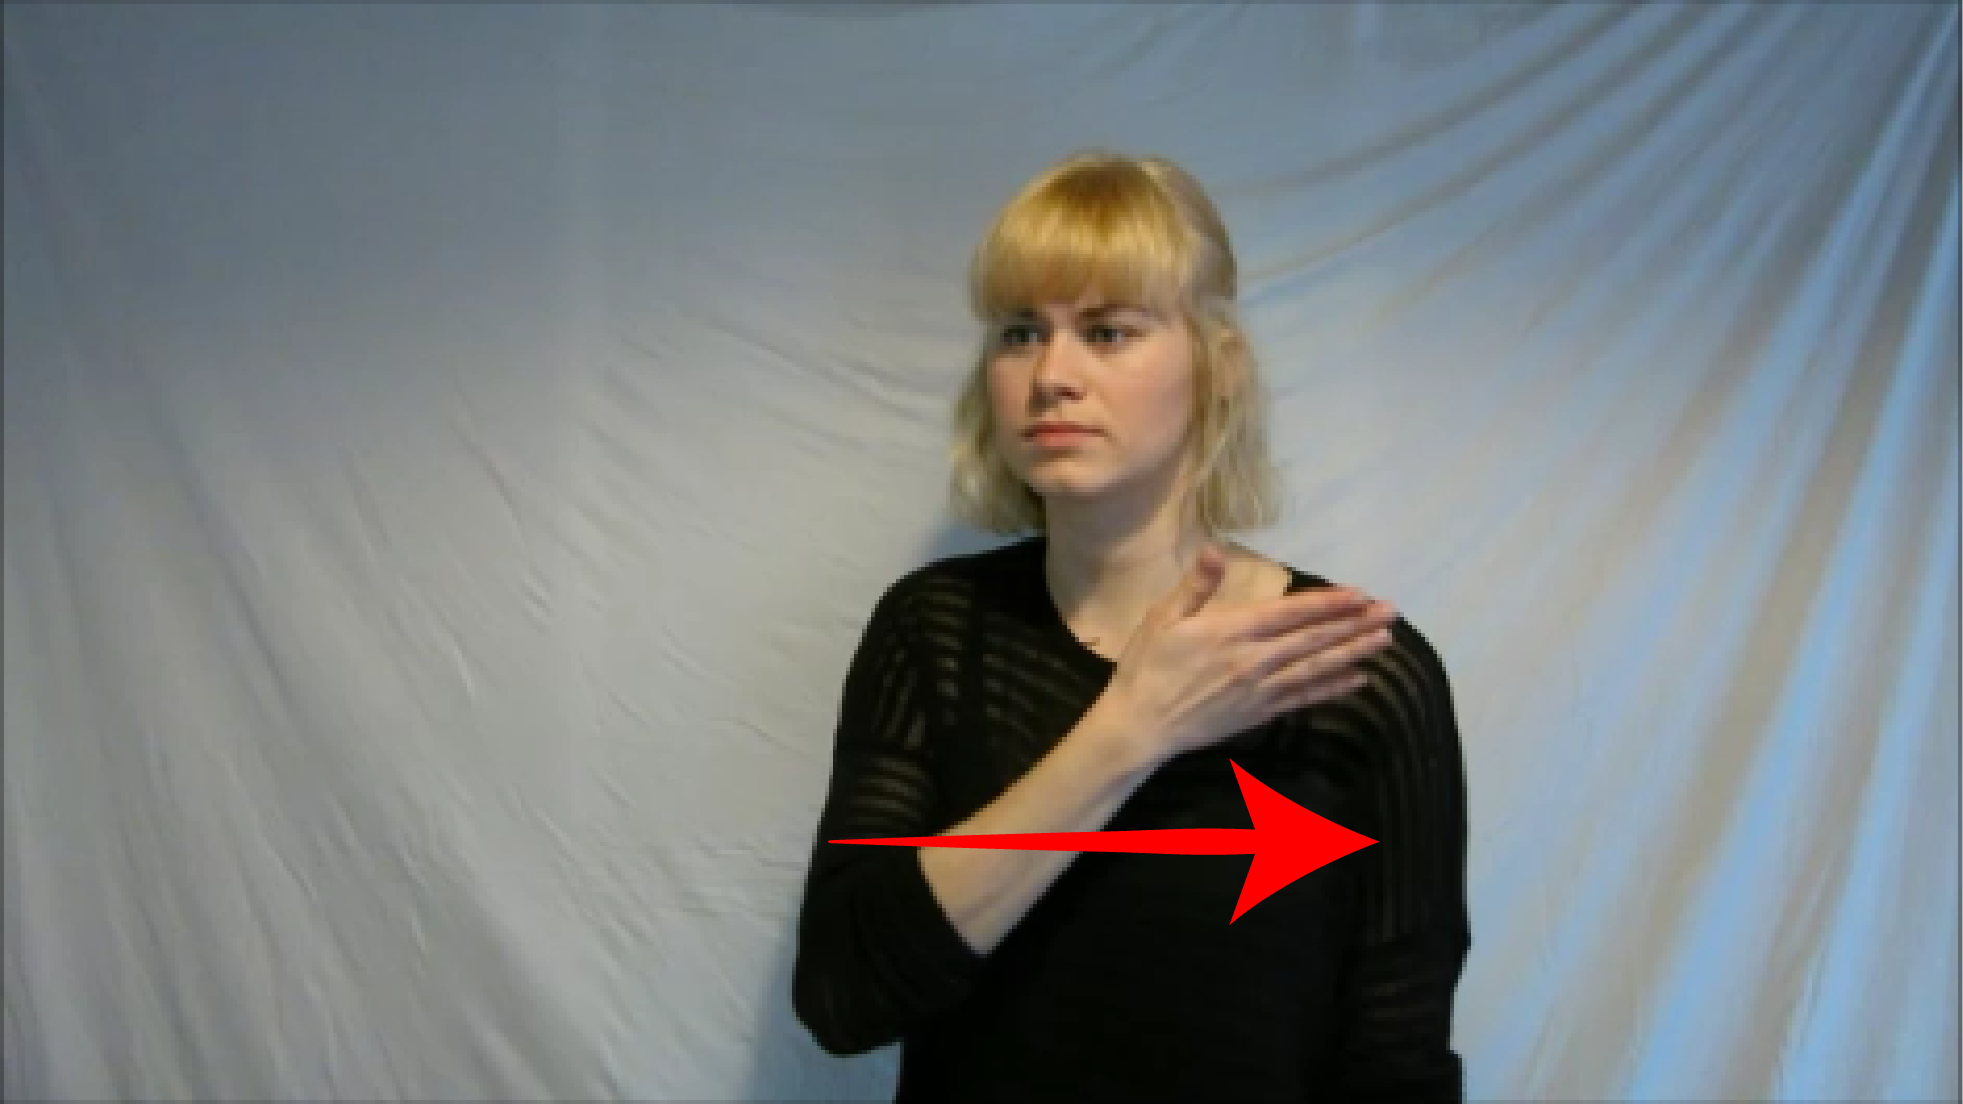
\includegraphics[resolution=300,width=\textwidth]{Flowdiagram/swipehoejretilvenstre-pil}
	\caption{Illustration af gestik-par 1; swipe fra højre mod venstre for at skifte til det næste musiknummer.}
	\label{fig:GestikPar1Skift}
\end{figure}
\noindent
% 
Sammenholdes udtalelserne fra de 10 testpersoner med hvad de rent faktisk gør så er der igen fire, som ikke formår at udføre bevægelsen i gestik-par 1 konsekvent. Testperson 1 skifter mellem at lave gestik-par 1 og gestik-par 5, når testpersonen referer til en swipe-bevægelse, men når testpersonen afslutningsvist bliver bedt om at gengive de fortrukne gestikker igen, så er er det gestik-par 1 testpersonen laver. Testperson 7 lægger ud med bedst at kunne lide gestik-par 7, hvorefter testpersonen ræsonnerer sig frem til at det istedet skal være gestik-par 1 med forbehold for at testpersonen foretrækker en mindre bevægelse. Når testpersonen afslutningsvist skal gengive sine fortrukne gestikker, så er det gestik-par 5 testpersonen laver, dog i den modsatte retning. Til at begynde med laver testperson 15 gestik-par 2 og når testpersonen taler om gestik-par 2, så er det egentlig gestik-par 1 testpersonen laver. Når testpersonen opfordres til at prøve gestikkerne til musik så bruger testpersonen både højre og venstre hånd, hvor begge bevægelser er modsat af hvad der foregår i gestik-par 1. Da testperson 15 afslutningsvist skal gengive sine fortrukne gestikker, så er det gestik-par 1, som testpersonen laver. Samme tendens forefindes ved testperson 16, som til at starte med laver gestik-par 1, men afslutningsvist så forklares og udføres bevægelsen, som i gestik-par 2. Testlederen gengiver gestik-par 1 for at være sikker på hvad testpersonen foretrækker og testpersonen giver udtryk for at det er sådan det skal være. Det tyder på at både testperson 15 og testperson 16 er i tvivl om hvilken retning swipe-bevægelsen skal være for enten at skifte til det næste eller forrige musiknummer. 

Ud af de 10 testpersoner har fire testpersoner forbedringer til gestik-par 1. Ifølge testperson 2 så skal det være ligegyldigt hvor mange fingre der bruges, da det er swipe-bevægelsen, der er essentielt. Det tyder derfor på at testpersonen ikke vil have noget imod at bruge gestik-par 5 til at skifte musiknummer, testpersonen har rangeret gestik-par 5 på en anden plads. Ifølge testperson 5 så er forbedringsforslaget at gøre bevægelsen til et ninja-hug, hvor fingrene samles, håndfladen peger opad og bevæges skrot ned fra højre mod venstre for at skifte til det næste musiknummer. For at skifte til det forrige musiknummer, foreslår testperson 5, igen at fingrene samles men denne gang skal håndfladen pege nedad og bevæges skrot ned fra venstre mod højre. Testperson 6, som påpegede et potentielt problem ved at skulle skifte til det forrige musiknummer og ikke bare genspille det nuværende musiknummer, foreslår at gestik-par 3 bruges til dette formål. Testperson 10's forbedringsforslag relaterer sig til at for at skifte til det næste musiknummer så skal højre hånd føres ind for foran kroppen og for at skifte til det forrige musiknummer skal venstre hånd føres ind foran kroppen.
%
\begin{figure}[H]
	\centering
	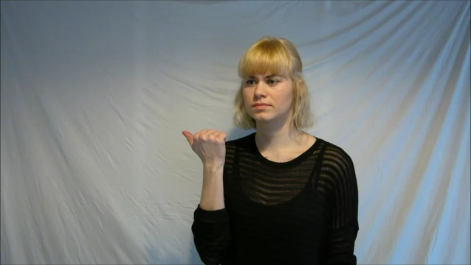
\includegraphics[resolution=300,width=\textwidth]{Flowdiagram/tommelfinger}
	\caption{Illustration af gestik-par 3; tommelfinger peger den retning musiknummeret skal skifte i.}
	\label{fig:GestikPar3Skift}
\end{figure}
\noindent
% 
Ud fra \autoref{tab:GestikParITopTreSkiftOversigt} fremgår det, at der kun er én testperson, som har tildelt gestik-par 3 en første plads. Gestik-par 3 illustreres på \autoref{fig:GestikPar3Skift}. Årsagen til at testperson 8 har valgt gestik-par 3 er fordi det er klart og tydeligt hvad der skal gøres. Foruden gestik-par 3 så har testperson 8 rangeret gestik-par 7 på en tredje plads, jævnfør \autoref{tab:GestikParITopTreSkift}, hvilket indikerer at testpersonen foretrækker en lille bevægelsesmængde. Når gestik-par 3 indgår på en anden plads, så er det i to ud af tre tilfælde efter gestik-par 1. Testperson 16 har rangeret gestik-par 3 over gestik-par 7 fordi den er mere diskret. Derudover pointerer testpersonen at de er nemme at udføre samt at det er de eneste to par, hvor der ikke skal en bevægelse til, hvilket ifølge testpersonen er ret smart. At det er nemt at udføre pointerer testperson 6 også. Gestik-par 3 rangeres på en tredje plads syv gange, hvor testperson 2 og testperson 5 har inkluderet parret i top tre enten fordi der ikke var andre, som kunne accepteres eller fordi det var det par, der kom tættest på en tredje plads. Det tyder ligeledes på at testperson 9 har brugt udelukkelses metoden og i forhold til gestik-par 3 kommenterer testpersonen at det er en meget lille bevægelse som er nem at overse. Testperson 10 giver udtryk for at årsagen til at gestik-par 3 inkluderes er fordi den er enorm simpel. Testperson 18 foretrækker både sin første og anden plads over gestik-par 3 da de er mere naturlige, men derudover kommenterer testpersonen at gestik-par 3 kan laves forholdvist passivt. Hverken testperson 4 eller testperson 7 forklarer hvorfor de har inkluderet gestik-par 3. 

I og med at der kun er en enkelt testperson, som har rangeret gestik-par 3 på en første plads og at det tyder på at største delen af de andre testpersoner, som har inkluderet gestik-par 3 har gjort det ud fra udelukkelsesmetoden og sammenholdt med \fullref{app:TestresultaterSkiftDaarlig}, hvor tre testpersoner har fravalgt gestik-par 3, så vurderes det at der belæg for at ekskludere gestik-par 3.
%
\begin{figure}[H]
	\centering
	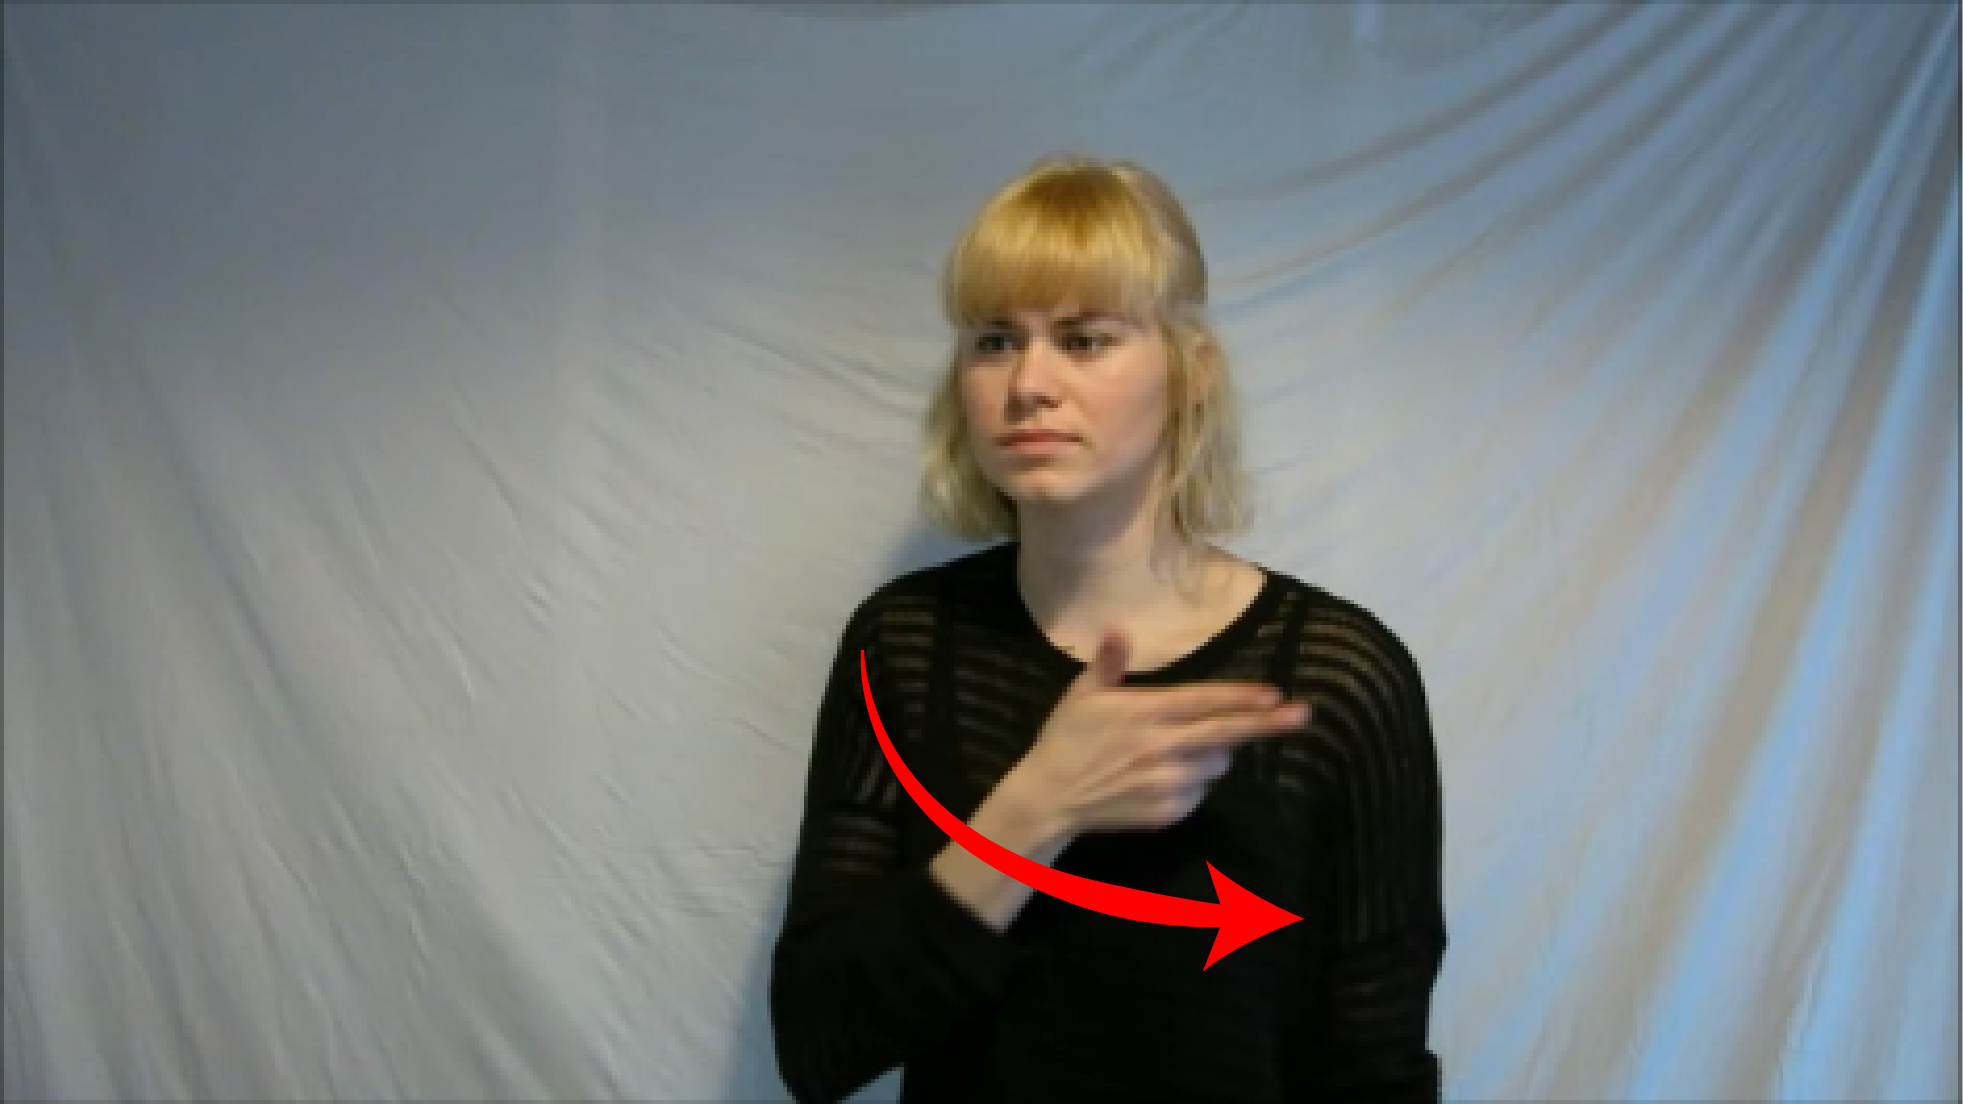
\includegraphics[resolution=300,width=\textwidth]{Flowdiagram/swipepegelangefingerhoejretilvenstre-pil}
	\caption{Illustration af gestik-par 5; swipe med pege- og langefinger fra højre mod venstre for at skifte til det næste musiknummer.}
	\label{fig:GestikPar5Skift}
\end{figure}
\noindent
%
Selvom gestik-par 5 kun er tildelt en første plads 3 gange, så indgår gestik-par 5 i testpersonernes samlede top tre ligeså ofte, som gestik par 1, jævnfør \autoref{tab:GestikParITopTreSkiftOversigt}. Gestik-par 5 er illustreret på \autoref{fig:GestikPar5Skift}. Testperson 9 giver udtryk for at de gestik-par, som indgår i top tre'en er valgt ud fra hvad testpersonen kunne huske og hvad der så mest elegant ud. I relation til gestik-par 5 kommenterer testperson 9 at det virkede mest logisk, men at det samtidig virkede pistolagtigt og at der var noget pege over det, uden at det blev et underviser-peg, hvor underviser-peget vurderes til at være negativt, jævnfør \autoref{fig:GestikPar5Skift}. Testperson 11 giver udtryk for at de gestik-par, som indgår i top tre'en er valgt ud fra hvad der er mindst naturligt i en samtale, hvorfor testpersonen har rangeret gestik-par 5 på en første plads. I forhold til gestik-par 5 vurderer testperson 11 at det giver intuitivt god mening at lave den bevægelse. Lignende synspunkter kommer til udtryk hos testperson 14, som igen vælger ud fra hvad der ikke føles naturligt og som testpersonen ikke vil komme til at lave ved en fejl, hvorfor et bestemt håndtegn er at foretrække. Desuden forbinder testperson 14 gestik-par 5 med en generel swipe-bevægelse, hvilket testpersonen finder naturligt. 

Tre ud af de syv testpersoner, testperson 1, testperson 2 og testperson 10, som har tildelt gestik-par 5, illustreret på \autoref{fig:GestikPar5Skift}, en anden plads gør det fordi det minder mest om gestik-par 1, illustreret på \autoref{fig:GestikPar1Skift}, som de alle tre har på en første plads. Årsagen til at testperson 10 har rangeret gestik-par 5 på en anden plads er udover, at det minder om gestik-par 1, så vurderer testpersonen at det er nødvendigt at tænke mere over gestik-par 5 i forhold til gestik-par 1. Det vurderes at testperson 4 ligeledes vælger gestik-par 5 fordi det minder mest om testpersonens første plads; gestik-par 2, så i det her tilfælde vælges gestik-par 5 kun hvis det fungerer efter samme princip, som i gestik-par 2. Hos testperson 3 går lignende tendenser igen, hvor testpersonen har tildelt gestik-par 5 en anden plads, fordi parret er næstmest naturligt, hvor gestik-par 1 er mest naturligt. Dog kommenterer testpersonen at det giver mere mening at bruge to fingre til at flytte på noget, jævnfør \autoref{fig:GestikPar5Skift}. Udover at testperson 5 giver udtryk for at gestik-par 5 er mere feminin sammenlignet med gestik-par 1, hvilket er årsagen til at gestik-par 5 tildeles en anden plads, så pointerer testpersonen, at gestik-par 5 tillader kontrol over hvad der skubbes til. Derudover tilføjer testperson 5 er gestik-par 5 er mindre voldsom og nemmere at udføre siddende end gestik-par 1. Testperson 13 giver udtryk for at fortrække gestikker hvor der både er bevægelse og hvor hånden skal være i et bestemt tegn, jævnfør \autoref{fig:GestikPar5Skift}, hvilket formentligt er årsagen til at gestik-par 1 ikke fremgår på top tre'en, jævnfør \autoref{tab:GestikParITopTreSkift}. Testperson 15, som har tildelt gestik-par 5 en tredje plads, giver udtryk for at gestik-par 1 er logisk og havde et mere simpelt tegn end de andre forslag. 

Af de 12 gange gestik-par 5 indgår på en top tre er der fire testpersoner, som ikke også har inkluderet gestik-par 1. Fokuseres der på hvad de fire testpersoner ellers har inkluderet i deres top tre, så er det kun testperson 4, som har inkluderet en statisk bevægelse; gestik-par 3, de tre andre har alle inkluderet gestik-par med en eller anden form for swipe-bevægelse, jævnfør \autoref{tab:GestikParITopTreSkift}. Endvidere er der kun fem testperson ud af de 12, som har inkluderet gestik-par 5 i deres top tre, som også har inkluderet en statisk gestik; gestik-par 3, illustreret på \autoref{fig:GestikPar3Skift}, og når det er tilfældet rangeres gestik-par 5 altid højere. Med udgangspunkt i det, samt testpersonernes udsagn så tyder det i høj grad på, at de fortrækker bevægelse, særligt en swipe-bevægelse som forbindes med interaktionen på en tablet eller en smartphone, såfremt der skal skiftes musiknummer. Derudover tyder det på at en af de største årsager til at testpersonerne hyppigst tildeler gestik-par 5 en anden plads er fordi det minder mest om gestik-par 1.

To af de tre testpersoner, som har tildelt gestik-par 5 en første plads, har givet et forbedringsforslag. Testperson 9 foreslår at bevægelsen laves med tre fremfor to fingre, for at undgå et pistolagtigt udtryk. Problemet ved at gøre det med tre fingre er, at det er svært og ubehageligt at strække ringefingeren samtidig med at lillefingeren skal bøjes, hvorfor dette forbedringsforslag afvises. Testperson 11's forbedringsforslag anses, ligesom ved gestik-par 1, som værende en selvfølge; forbedringen ifølge testperson 11 er at bevægelsesmængden reduceres så det eksempelvis er muligt at skifte musiknummer med en swipe-bevægelse fra håndleddet.
%
\begin{figure}[H]
	\centering
	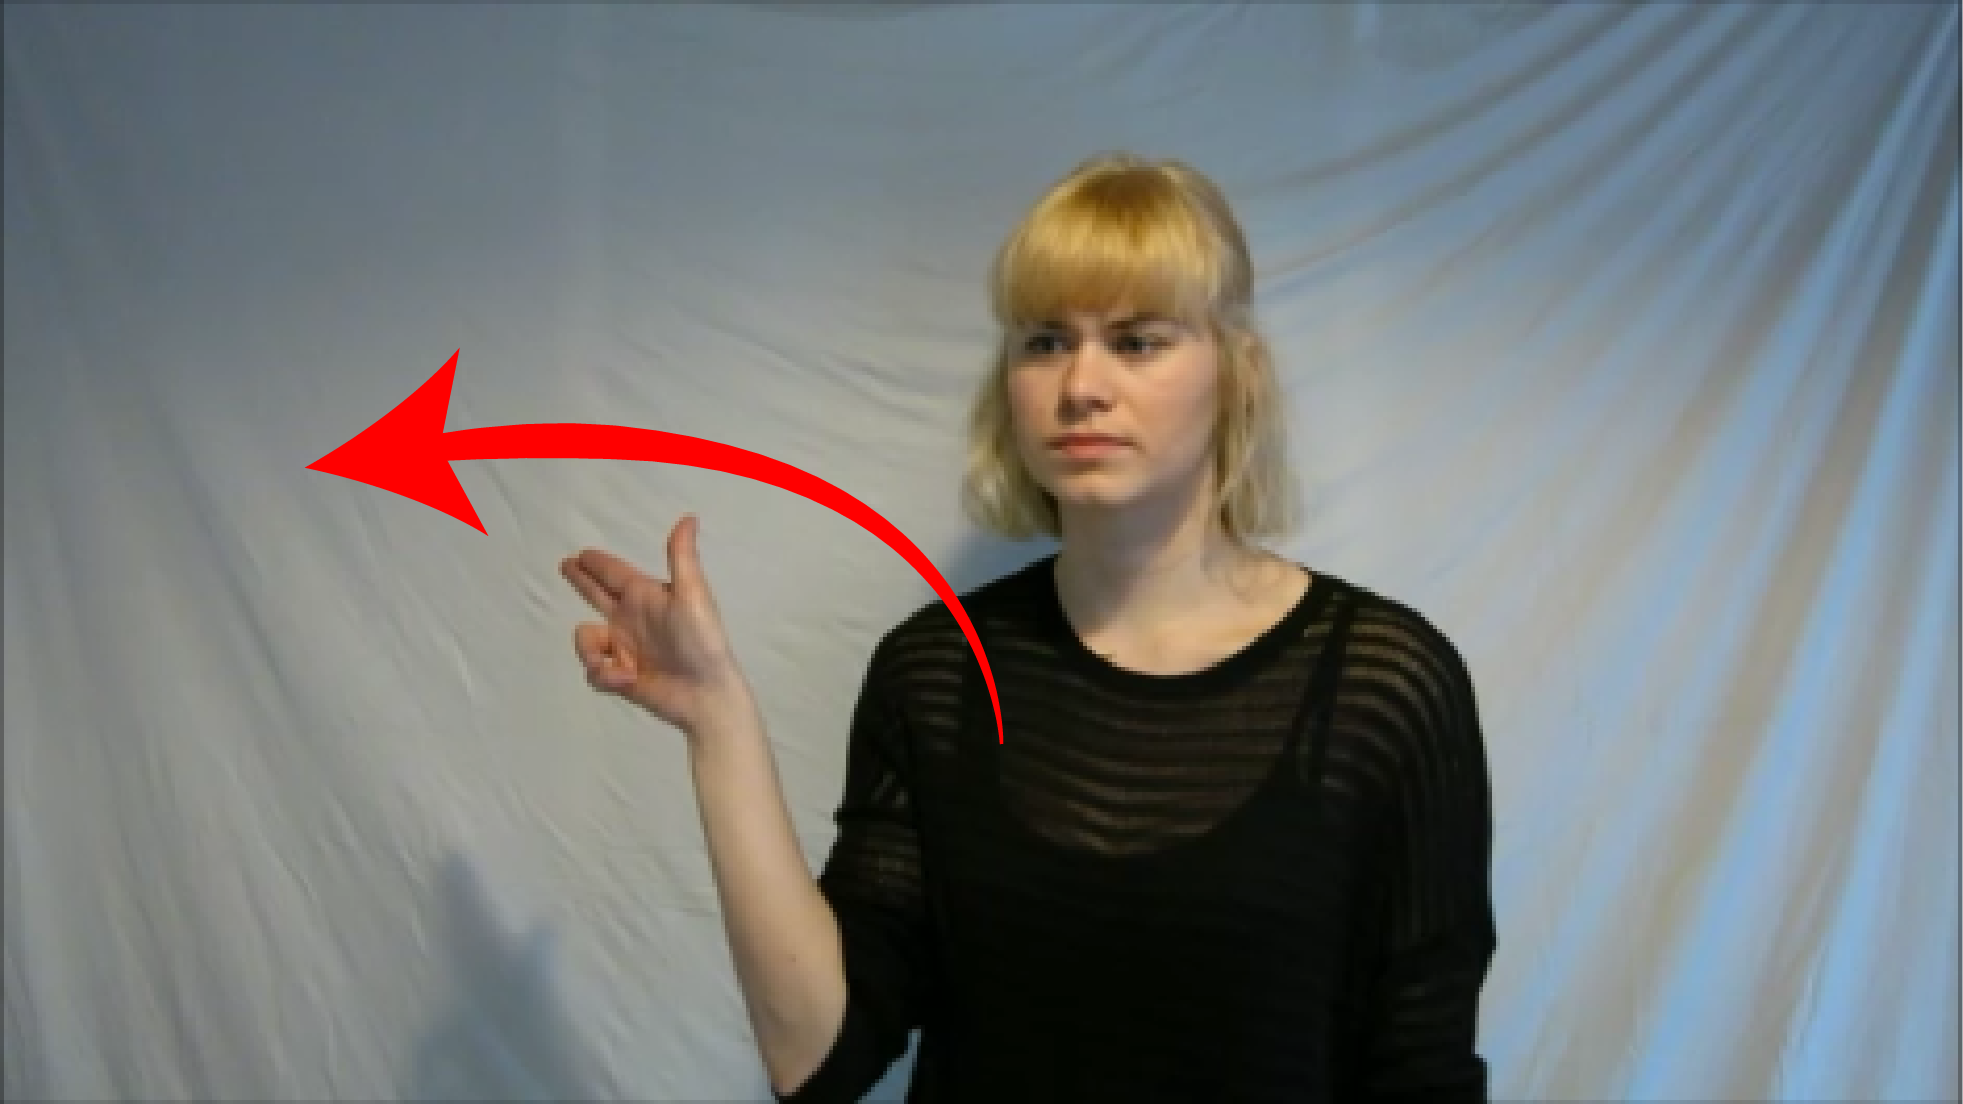
\includegraphics[resolution=300,width=\textwidth]{Flowdiagram/pegelangefingerpegebue-pil}
	\caption{Illustration af gestik-par 6; bue med pege- og langefinger fra venstre mod højre for at skifte til det næste musiknummer.}
	\label{fig:GestikPar6Skift}
\end{figure}
\noindent
%                
Gestik-par 6 er kun tildelt en første plads én gang; af testperson 13, jævnfør \autoref{tab:GestikParITopTreSkift}. Gestik-par 6 illustreres på \autoref{fig:GestikPar6Skift}. Testpersonen formår ikke at præcisere hvorfor gestik-par 6 rangeres højere end gestik-par 5, men testpersonen giver udtryk for bedst at kunne lide de gestikker hvor hånden bevæges på en bestemt måde samt de gestikker, som indeholder et specielt håndtegn, jævnfør \autoref{fig:GestikPar5Skift} og \autoref{fig:GestikPar6Skift}. I de to tilfælde hvor gestik-par 6 indgår på en anden plads, så er det efter gestik-par 5, hvor det ud fra testpersonernes udsagn vurderes at det skyldes dels håndtegnet og dels bevægelsen. Når gestik-par 6 indgår på en tredje plads så har testpersonerne i begge tilfælde tildelt gestik-par 1 en første plads og enten gestik-par 5 eller gestik-par 3 en anden plads. 

I og med at der kun er en testperson, som har tildelt gestik-par 6 en første plads og det tilmed vurderes at når gestik-par 6 indgår enten på en anden eller tredje plads, så er testpersonernes ønsker dækket af et eller flere af de gestik-par, som de har rangeret over, så vurderes det at der er belæg for at ekskludere gestik-par 6.\blankline
%
Baseret på foregående analyse samt \fullref{app:TestresultaterSkiftDaarlig} hvor i alt fem gestik-par er ekskluderet, så står valget mellem gestik-par 1 og gestik-par 5. Fælles for de to gestik-par er at de indgår lige mange gange i testpersonernes samlede top tre; 12 gange i alt, selvom gestik-par 1 indgår 10 gange og gestik-par 5 kun indgår tre gange. Det tyder på at de testpersoner, som har rangeret gestik-par 1 over gestik-par 5 giver udtryk for, at der egentlig ikke er så stor forskel mellem de to og at årsagen til at gestik-par 5 tildeles en anden plads frem for de resterende forslag skyldes at det minder mest om gestik-par 1. Derudover pointere flere testpersoner, som ikke nødvendigvis har rangeret gestik-par 1 over gestik-par 5, at de foretrækker dels at gestikken indeholder en bevægelse og dels at der er knyttet et bestemt håndtegn til gestikken. Ydermere er der flere testpersoner, som begår fejl når de udfører gestik-par 1, hvorimod ingen testpersoner begår fejl når de udfører gestik-par 5. Endvidere påpeger flere testpersoner at bevægelsen i gestik-par 1 er naturlig, hvorfor det antages at bevægelsen formentlig forekommer i ubevidst i deres kropssprog. I tillæg vurderes det, at størstedelen af de egenskaber testpersonerne foretrækker ved gestik-par 1 går igen i gestik-par 5. Tages alt dette i betragtning vurderes det at der er belæg for at knytte gestik-par 5 til at skifte musiknummer.          

